%
Figure \ref{fig:a_rover} shows (top to bottom)
the three types of access intervals:
access-use, useful-lifetime, and def-use.
For each type of access interval, the data for each of the
ten benchmark programs are overlaid on the same graph.
For each access interval type, both a density 
and a distribution is provided.
%
\begin{figure}[tb]
\centering
\epsfig{file=a_rover.eps,width=6.5in}
\caption{{\em Register Access Intervals.} 
Data results for all programs are shown overlaid.
The density is shown on the left and the distribution is shown
on the right.
All intervals are measured in dynamic numbers of executed instructions.}
\label{fig:a_rover}
\end{figure}
%
As can be seen from the graphs of Figure \ref{fig:a_rover},
all of the benchmark programs perform similarly and have
rather short (40 or less) interval lengths for most of each type
of access interval.
%
